% ===========================================================================
%  ______          _           _     ______           _
%  | ___ \        (_)         | |   |___  /          | |
%  | |_/ / __ ___  _  ___  ___| |_     / /  ___ _ __ | |__  _   _ _ __
%  |  __/ '__/ _ \| |/ _ \/ __| __|   / /  / _ \ '_ \| '_ \| | | | '__|
%  | |  | | | (_) | |  __/ (__| |_  ./ /__|  __/ |_) | | | | |_| | |
%  \_|  |_|  \___/| |\___|\___|\__| \_____/\___| .__/|_| |_|\__, |_|
%                _/ |                          | |           __/ |
%               |__/                           |_|          |___/
%
%                       Main Document Project Zephyr
% ===========================================================================
%
%   Needed ArchLinux Packaes:
%
%   texlive-bin
%   texlive-core
%   texlive-fontsextra
%   texlive-bibtexextra
%   texlive-genericextra
%   texlive-latexextra
%   texlive-publishers
%

%---------------------------------------------------------------------------
\documentclass[
    a4paper,                                                % paper format
    10pt,                                                   % fontsize
    twoside,                                                % double-sided
    openright,                                              % begin new chapter on right side
    notitlepage,                                            % use no standard title page
    parskip=half,                                           % set paragraph skip to half of a line
]{scrreprt}
%---------------------------------------------------------------------------

\raggedbottom
\KOMAoptions{cleardoublepage=plain}                         % Add header and footer on blank pages


% Load Standard Packages:
%---------------------------------------------------------------------------
\usepackage[standard-baselineskips]{cmbright}
\usepackage[ngerman]{babel}                                 % german hyphenation
\usepackage[ansinew]{inputenc}                              % Windows - load extended character set (ISO 8859-1)
\usepackage[T1]{fontenc}                                    % hyphenation of words with ���
\usepackage{textcomp}                                       % additional symbols
\usepackage{ae}                                             % better resolution of Type1-Fonts
\usepackage{fancyhdr}                                       % simple manipulation of header and footer
\usepackage{etoolbox}                                       % color manipulation of header and footer
\usepackage{graphicx}                                       % integration of images
\usepackage{float}                                          % floating objects
\usepackage{caption}                                        % for captions of figureMain documents and tables
\usepackage{booktabs}                                       % package for nicer tables
\usepackage{tocvsec2}                                       % provides means of controlling the sectional numbering
\usepackage{listings}                                       % Highlight aaaall the codes!

\usepackage[]{acronym}                                      % Glossary
\usepackage[acronym,toc]{glossaries}
%---------------------------------------------------------------------------

% Load Math Packages
%---------------------------------------------------------------------------
\usepackage{amsmath}                                        % various features to facilitate writing math formulas
\usepackage{amsthm}                                         % enhanced version of latex's newtheorem
\usepackage{amsfonts}                                       % set of miscellaneous TeX fonts that augment the standard CM
\usepackage{amssymb}                                        % mathematical special characters
\usepackage{exscale}                                        % mathematical size corresponds to textsize
%---------------------------------------------------------------------------

% Package to facilitate placement of boxes at absolute positions
%---------------------------------------------------------------------------
\usepackage[absolute]{textpos}
\setlength{\TPHorizModule}{1mm}
\setlength{\TPVertModule}{1mm}
%---------------------------------------------------------------------------

% Definition of Colors
%---------------------------------------------------------------------------
\RequirePackage{color}                                      % Color (not xcolor!)
\definecolor{orange}{RGB}{244, 182, 66}
\definecolor{purple}{RGB}{188, 66, 244}
\definecolor{linkblue}{rgb}{0,0,0.8}                        % Standard
\definecolor{darkblue}{rgb}{0,0.08,0.45}                    % Dark blue
\definecolor{bfhgrey}{rgb}{0.41,0.49,0.57}                  % BFH grey
\definecolor{linkcolor}{rgb}{0,0,0.8}                       % Blue for the web- and cd-version!
\definecolor{linkcolor}{rgb}{0,0,0}                         % Black for the print-version!
\definecolor{codebackground}{RGB}{196, 218, 255}            % Codehighlight background
%---------------------------------------------------------------------------

% Codehighlightings
%---------------------------------------------------------------------------
\lstdefinestyle{BashInputStyle}{
    belowcaptionskip=1\baselineskip,
    breaklines=true,
    frame=tb,
    numbers=left,
    numberstyle=\tiny,
    linewidth=0.95\linewidth,
    xleftmargin=0.05\linewidth,
    language=bash,
    showstringspaces=false,
    basicstyle=\small\sffamily,
    keywordstyle=\bfseries\color{black},
    backgroundcolor=\color{codebackground},
}

\lstdefinestyle{customc}{
    belowcaptionskip=1\baselineskip,
    breaklines=true,
    frame=tb,
    numbers=left,
    numberstyle=\tiny,
    linewidth=0.95\linewidth,
    xleftmargin=0.05\linewidth,
    language=C,
    showstringspaces=false,
    basicstyle=\footnotesize\ttfamily,
    keywordstyle=\bfseries\color{black},
    backgroundcolor=\color{codebackground},
    commentstyle=\itshape\color{purple},
    identifierstyle=\color{blue},
    stringstyle=\color{orange},
}
%---------------------------------------------------------------------------

% Hyperref Package (Create links in a pdf)
%---------------------------------------------------------------------------
\usepackage[
    pdftex,ngerman,bookmarks,plainpages=false,pdfpagelabels,
    backref = {false},                                      % No index backreference
    colorlinks = {true},                                    % Color links in a PDF
    hypertexnames = {true},                                 % no failures "same page(i)"
    bookmarksopen = {true},                                 % opens the bar on the left side
    bookmarksopenlevel = {0},                               % depth of opened bookmarks
    pdftitle = {Projekt Zephyr},                            % PDF-property
    pdfauthor = {schma5},                                   % PDF-property
    pdfsubject = {LaTeX Bericht},                           % PDF-property
    linkcolor = {linkcolor},                                % Color of Links
    citecolor = {linkcolor},                                % Color of Cite-Links
    urlcolor = {linkcolor},                                 % Color of URLs
]{hyperref}
%---------------------------------------------------------------------------

% Set up page dimension
%---------------------------------------------------------------------------
\usepackage{geometry}
\geometry{
    a4paper,
    left=28mm,
    right=15mm,
    top=30mm,
    headheight=20mm,
    headsep=10mm,
    textheight=242mm,
    footskip=15mm
}
%---------------------------------------------------------------------------

% Makeindex Package
%---------------------------------------------------------------------------
\usepackage{makeidx}                                        % To produce index
\makeindex                                                  % Index-Initialisation
%---------------------------------------------------------------------------

% Glossary Package
%---------------------------------------------------------------------------
\makeglossaries
%---------------------------------------------------------------------------

% Intro:
%---------------------------------------------------------------------------
\begin{document}                                            % Start Document
\settocdepth{section}                                       % Set depth of toc
\pagenumbering{roman}
%---------------------------------------------------------------------------

\providecommand{\titel}{Zephyr-Projekt}		% Titel der Projektarbeit                                      % Titel der Arbeit aus Datei titel.tex lesen
\providecommand{\versionnumber}{0.1}			%  Aktuelle Versionsnummer eingeben
\providecommand{\versiondate}{29.09.2016}		%  Datum der aktuellen Version eingeben                                    % Versionsnummer und -datum aus Datei version.tex lesen

% Set up header and footer
%---------------------------------------------------------------------------
\makeatletter
\patchcmd{\@fancyhead}{\rlap}{\color{bfhgrey}\rlap}{}{}     % new color of header
\patchcmd{\@fancyfoot}{\rlap}{\color{bfhgrey}\rlap}{}{}     % new color of footer
\makeatother

\fancyhf{}                                                  % clean all fields
\fancypagestyle{plain}{                                     % new definition of plain style
    \fancyfoot[OR,EL]{\footnotesize \thepage}               % footer right part --> page number
    \fancyfoot[OL,ER]{\footnotesize \titel, Version \versionnumber, \versiondate} % footer even page left part
}

\renewcommand{\chaptermark}[1]{\markboth{\thechapter. #1}{}}
\renewcommand{\headrulewidth}{0pt}                          % no header stripline
\renewcommand{\footrulewidth}{0pt}                          % no bottom stripline

\pagestyle{plain}
%---------------------------------------------------------------------------


% Title Page and Abstract
%---------------------------------------------------------------------------
%
% Project documentation template
% ===========================================================================


\begin{titlepage}


% BFH-Logo absolute placed at (28,12) on A4 and picture (16:9 or 15cm x 8.5cm)
% Actually not a realy satisfactory solution but working.
%---------------------------------------------------------------------------
\setlength{\unitlength}{1mm}
\begin{textblock}{20}[0,0](28,12)
	
\includegraphics[scale=1.0]{bilder/BFH_Logo_B.png}
\end{textblock}

\begin{textblock}{154}(28,48)
	\begin{picture}(150,2)
		\put(0,0){\color{bfhgrey}\rule{150mm}{2mm}}
	\end{picture}
\end{textblock}

\begin{textblock}{154}[0,0](28,50)
	
\includegraphics[scale=1.0]{bilder/Zephyr-Project.jpg}			% Titelbild definieren
\end{textblock}

\begin{textblock}{154}(28,135)
	\begin{picture}(150,2)
		\put(0,0){\color{bfhgrey}\rule{150mm}{2mm}}
	\end{picture}
\end{textblock}
\color{black}

% Institution / Titel / Untertitel / Autoren / Experten:
%---------------------------------------------------------------------------
\begin{flushleft}

\vspace*{115mm}

\fontsize{26pt}{28pt}\selectfont 
\titel 				\\							% Titel aus der Datei vorspann/titel.tex lesen
\vspace{2mm}

\fontsize{16pt}{20pt}\selectfont\vspace{0.3em}
Echtzeit-OS f�r das Internet der Dinge 			\\							% Untertitel eingeben
\vspace{5mm}

\fontsize{10pt}{12pt}\selectfont
\textbf{Projektarbeit} \\									% eingeben
\vspace{3mm}

% Abstract (eingeben):
%---------------------------------------------------------------------------
\begin{textblock}{150}(28,190)
\fontsize{10pt}{12pt}\selectfont
Die Linux Foundation hat mit dem Projekt Zephyr mit der Entwicklung eines Echtzeit-Betriebssystems f�r das Internet der Dinge (IoT) begonnen.
Zephyr ist ein Open-Source-Betriebssystem mit dem Ziel ein solides OS f�r IoT Ger�te mit geringen Ressourcen bereitzustellen. Es nutzt eine echtzeitf�hige Kombination aus Nano- und Microkernel. 
Im Gegensatz zu einem Linux Kernel ben�tigt Zephyr nur zwischen 8 und 512 KByte an Arbeitsspeicher.  Aktuell werden folgenden Plattformen unterst�tzt: x86, ARM und ARC EM4
\end{textblock}

\begin{textblock}{150}(28,225)
\fontsize{10pt}{17pt}\selectfont
\begin{tabbing}
xxxxxxxxxxxxxxx\=xxxxxxxxxxxxxxxxxxxxxxxxxxxxxxxxxxxxxxxxxxxxxxx \kill
Studiengang:	\> Elektro- und Kommunikationstechnik			\\
Autoren:		\> Aaron Schmocker, David Wyss					\\
Betreuer:		\> Martin Aebersold								\\
Auftraggeber:	\> Martin Aebersold								\\
Experten:		\> Martin Aebersold								\\
Datum:			\> \versiondate									\\
\end{tabbing}

\end{textblock}
\end{flushleft}

\begin{textblock}{150}(28,280)
\noindent 
\color{bfhgrey}\fontsize{9pt}{10pt}\selectfont
Berner Fachhochschule | Haute �cole sp�cialis�e bernoise | Bern University of Applied Sciences
\color{black}\selectfont
\end{textblock}


\end{titlepage}

%
% ===========================================================================
% EOF
%
                      % activate for Titelseite mit Bild
% Versionenkontrolle :
% -----------------------------------------------

\begin{textblock}{180}(15,150)
\color{black}
\begin{huge}
Versionen
\end{huge}
\vspace{10mm}

\fontsize{10pt}{18pt}\selectfont
\begin{tabbing}
xxxxxxxxxxx\=xxxxxxxxxxxxxxx\=xxxxxxxxxxxxxx\=xxxxxxxxxxxxxxxxxxxxxxxxxxxxxxxxxxxxxxxxxxxxxxx \kill
Version	\> Datum	\> Status		\> Bemerkungen \\
0.1	\> 29.09.2016	\> Entwurf		\> Titelblatt erstellt und Template f�r Linux angepasst \\	
%0.2	\> 21.08.2016	\> Entwurf		\> Phasellus scelerisque \\ 
%0.3	\> 02.09.2016	\> Entwurf		\> Donec eget aliquam urna. Lorem ipsum dolor sit amet \\ 
%1.0	\> 12.09.2016	\> Definitiv	\> Lorem ipsum dolor sit ametPhasellus scelerisque, leo sed iaculis ornare \\ 
%1.1	\> 04.11.2016	\> Korrektur	\> Layout angepasst \\
%1.2	\> 01.02.2016	\> Erg�nzung	\> Kapitel 1.1 erweitert \\
\end{tabbing}

\end{textblock}

\cleardoubleemptypage
\setcounter{page}{1}
\cleardoublepage
\phantomsection 
\addcontentsline{toc}{chapter}{Management Summary}
\chapter*{Management Summary}
\label{chap:managementSummary}

Lorem ipsum dolor sit amet, consectetur adipiscing elit. Phasellus scelerisque, leo sed iaculis ornare, mi leo semper urna, ac elementum libero est at risus. Donec eget aliquam urna. Lorem ipsum dolor sit amet, consectetur adipiscing elit. Nunc fermentum nunc sollicitudin leo porttitor volutpat. Duis ac enim lectus, quis malesuada lectus. Aenean vestibulum suscipit justo, in suscipit augue venenatis a. Donec interdum nibh ligula. Aliquam vitae dui a odio cursus interdum quis vitae mi. Phasellus ornare tortor fringilla velit accumsan quis tincidunt magna eleifend. Praesent nisl nibh, cursus in mattis ac, ultrices ac nulla. Nulla ante urna, aliquet eu tempus ut, feugiat id nisl. Nunc sit amet mauris vitae turpis scelerisque mattis et sed metus. Aliquam interdum congue odio, sed semper elit ullamcorper vitae. Morbi orci elit, feugiat vel hendrerit nec, sollicitudin non massa. Quisque lacus metus, vulputate id ullamcorper id, consequat eget orci \nocite{kopka:band1} \nocite{Marti06}. 

\cleardoubleemptypage
%---------------------------------------------------------------------------

% Table of contents
%---------------------------------------------------------------------------
\tableofcontents
\cleardoublepage
%---------------------------------------------------------------------------

% Main part:
%---------------------------------------------------------------------------
\pagenumbering{arabic}

% !TeX encoding = ISO-8859-1
\chapter{Einleitung}
\label{chap:einleitung}

\section{TEST}

\section{TEST2}



% !TeX encoding = ISO-8859-1
\chapter{ZephyrOverview}
\label{chap:overview}

\section{�bersicht �ber Zephyr}

Zephyr ist ein Open-Source-Echtzeitbetriebssystem f�r das Internet der Dinge. Die Architektur basiert auf einer echtzeitf�higen Kombination von 
Es wird aktuell von der LinuxFoundation in Zusammenarbeit mit den Firmen Intel, NXP und Synopsys in der Form eines Collaborative Projects entwickelt. Dadurch soll versucht werden die bei der Linux- und Open-Source-Entwicklung verwendeten Arbeitsweisen und Ideen auch im Bereich der Industrie einzubringen. [1]
Ziel ist es ein robustes und sicheres Betriebsystem f�r das Internet der Dinge zu schaffen. Zephyr ist vollst�ndig Open-Source steht unter der Apache Lizenz Version 2.0. [2] 
Dieses Lizenzierungsmodell kommt Firmen und Unternehmen entgegen welche den Einsatz von Open-Source-Software scheuen welche unter der GPL (Gnu Public License) stehen. [2] Wird in Produkten Software verwendet welche unter GPL lizensiert ist, zwingt dieses Lizenzmodell die Firmen dazu ihre Produkte ebenfalls unter GPL zu ver�ffentlichen. Dies beinhaltet auch s�mltiche �nderungen welche vorgenommen wurden. Bei der Apache-Lizenz ist dies nicht zwingend. [3]
Momentan unterst�tzt der Zephyr-Kernel Prozessoren der Architekturen ARC, ARM-v7 aber auch x86. Dadurch ist das System auf popul�ren Plattformen wie dem Arduino 101 Board, dem Arduino Due Board, dem NXP Freedom DK lauff�hig und Intel Galileo Gen 2. Zur Kommunikation stehen unter anderem Protokolle Ipv4, Ipv6, Bluetooth 4.0, 6LoWPAN zur verf�gung. [4]

Sources:
 %https://www.linuxfoundation.org/news-media/announcements/2016/02/linux-foundation-announces-project-build-real-time-operating-system
 %https://www.heise.de/newsticker/meldung/Zephyr-Linux-Foundation-startet-Projekt-fuer-IoT-Betriebssystem-ohne-Linux-3109906.html?wt_mc=rss.ho.beitrag.atom
 %http://www.apache.org/licenses/LICENSE-2.0
 %https://www.zephyrproject.org/doc/board/board.html

\section{Ziele}

Zephyr ist f�r den Einsatz auf Ger�ten mit geringem Speicherplatz und feststehender Hardwarekonfiguration gedacht. Darunter fallen unter anderem Steuerungen f�r Heizungs- und Beleuchtungssysteme aber auch Ger�te aus allen Bereichen des t�glichen Lebens mit Internet-Anbindung.

Das ZephyrProjekt verfolgt laut [1] folgende Ziele:
\begin{itemize}
    \item Kleiner footprint - lauff�hig mit minimal 10kB
    \item CPU unabh�ngige Architektur
    \item Modular und Skalierbar
    \item Hoche Sicherheitsstandards
    \item Unterst�tzt von Grund auf viele unterschiedliche Boards und Kommunikationsprotokolle
    \item M�chtige Entwicklungswerkzeuge
    \item OpenSource Kernel mit Apache v2.0 Lizenz
\end{itemize}

 %http://hackerboards.com/zephyr-a-tiny-open-source-iot-rtos/

\section{Aufbau}

Das Zephyr OS setzt auf eine Kombination von Nano- und Mikrokernel. Dadurch soll Zephyr  bereits mit nur 10 Kbyte an Speicherplatz lauff�hig sein. Das macht Zephyr besonders f�r Anwendungen auf kleinen Mikrokontrollern attraktiv. Bei einem herk�mmlichen Linux-Kernel w�re dies nicht denkbar. G�ngige Adaptionen f�r Smartphone SoCs ben�tigen laut [1] in der kleinsten Konfiguration noch bis zu 200KB RAM und rund 1MB Flash.

Der Nanokernel bietet Echtzeit-F�higkeiten. Die Zeit die der Nanokernel f�r die Abarbeitung einer Aufgabe ben�tigt ist also deterministisch. Dies unabh�ngig davon wie stark das System gerade ausgelastet ist. F�r alle Aufgaben welche keine Anforderungen an Echtzeit-Verarbeitung stellen verf�gt das System �ber einen Microkernel. 
[1] http://linuxdevices.linuxgizmos.com/my-linux-is-smaller-than-your-linux-a/

\section{Aufsetzen der SDK unter Ubuntu}
\section{Vergleich mit anderen RTOS}
\section{Sicherheitsaspekte}
\section{Portierungsaufwand}
 % !TeX encoding = ISO-8859-1
 \chapter{FreeRTOS-Overview}
 \label{chap:overview}
 
 \section{�bersicht �ber FreeRTOS}
 
 FreeRTOS ist laut Beschreibung der Real Time Enginners Ltd \cite{LinuxFoundation} ein Open-Source-Echtzeitbetriebssystem. FreeRTOS wurde professionell entwickelt und wird gewartet durch die Firma Real Time Enginners Ltd. Sie arbeiten seit �ber 12 Jahren in enger Partnerschaft mit weltweit f�hrenden Chip-Herstellern zusammmen, um ihren Kunden eine v�llig freie Qualit�tssoftware zur Verf�gung zu stellen. Mittels hohem C Quellcodes Standart wurde das robuste Echtzeitbetriebssystem zum Marktf�hrer unter den RTOS und unterst�tz �ber 35 Architekturen.
 
 FreeRTOS ist sehr streng verwaltet, nicht nur in Software-Coding-Standards und Look-and-Feel, sondern auch in der Umsetzung. Beispielsweise:
 
  \begin{itemize}
  	\item  FreeRTOS f�hrt nie einen nicht-deterministischen Vorgang aus, wie etwa das Verfolgen einer verkn�pften Liste, und zwar innerhalb eines kritischen Abschnitts oder Interrupts.
  	\item Wir sind besonders stolz auf die effiziente Software-Timerimplementierung, die keine CPU-Zeit in Anspruch nimmt, es sei denn, ein Timer muss tats�chlich gewartet werden. Software-Timer enthalten keine Variablen, die bis auf Null gez�hlt werden m�ssen.
  	\item Ebenso ben�tigen Listen von blockierten (angeh�ngten) Tasks keine zeitraubende periodische Wartung.
  	\item Direkt zu Task-Benachrichtigungen erm�glichen eine schnelle Task-Signalisierung mit praktisch keinem RAM-Overhead und k�nnen in der Mehrzahl der Inter-Task- und Interrupt-Task-Signaling-Szenarien verwendet werden.
  	\item Das FreeRTOS-Warteschlangen-Nutzungsmodell schafft es, Einfachheit mit Flexibilit�t (in einer winzigen Codegr��e) zu kombinieren - Attribute, die sich normalerweise gegenseitig ausschlie�en.
  \end{itemize}
 
  
  \begin{figure}[h]
  	\centering
  	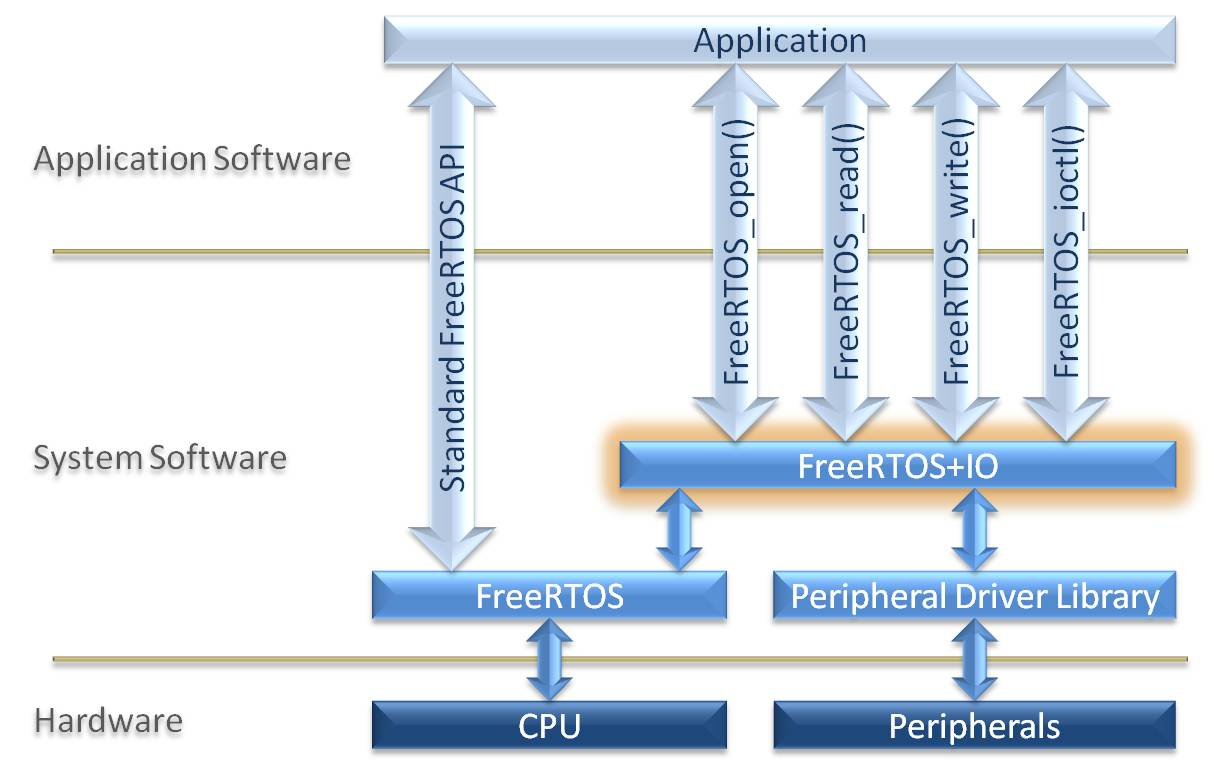
\includegraphics[width=0.7\linewidth]{bilder/FreeRTOS_Context.jpg}
  	\caption{�bersicht �ber das FreeRTOS}
  	\label{fig:components}
  \end{figure}
  \vspace{10mm}
 
Es wird unter der GPL mit einer zus�tzlichen Einschr�nkung und optionaler Ausnahme verteilt. Die Einschr�nkung verbietet das Benchmarking, w�hrend die Ausnahme erlaubt, dass der propriet�re Code der Benutzer eine geschlossene Quelle bleibt, w�hrend der Kernel selbst als Open Source beibehalten wird, wodurch die Verwendung von FreeRTOS in propriet�ren Anwendungen erleichtert wird. FreeRTOS wurde schon im Weltraum eingesetzt.\cite{FreeRTOSProjectDocumentation}
 
 \section{Ziele}
 
 Die urspr�ngliche Aufgabe des FreeRTOS-Projekts war es, eine kostenlose RTOS-L�sung bereitzustellen, die einfach zu bedienen war. Das heisst, einfach zu erstellen und zu implementieren, auf einem Windows- oder Linux Computer, ohne herauszufinden, welche Quelldateien erforderlich sind und welche Pfade erforderlich sind, oder wie die Echtzeit-Debugging-Umgebung konfiguriert wird. Dies wurde durch die Bereitstellung von vorkonfigurierten Beispielprojekten f�r jeden offiziell unterst�tzten Board erreicht.
 
 FreeRTOS ist ein skalierbarer Echtzeitkern, der speziell f�r kleine Embedded-Systeme entwickelt wurde. Zu den Highlights geh�ren:\cite{FreeRTOSProjectDocumentation}
 
 
 \begin{itemize}
 	\item Freier RTOS-Scheduler - pr�ventive, kooperative und hybride Konfigurationsoptionen mit optionalem Time Slicing
 	\item CPU unabh�ngige Architektur
 	\item SafeRTOS-Produkt soll ein hohes Ma� an Vertrauen in die Codeintegrit�t schaffen
 	\item Enth�lt einen Tickless-Modus f�r Anwendungen mit geringer Leistung
 	\item Unterst�tzt viele unterschiedliche Boards und Kommunikationsprotokolle
 	\item RTOS-Objekte (Tasks, Warteschlangen, Semaphoren, Software-Timer, Mutexes und Ereignisgruppen) k�nnen entweder mit dynamisch oder statisch zugewiesenem RAM erstellt werden
 	\item Unterst�tzt sowohl Echtzeitaufgaben als auch Co-Routinen.
 	\item Mutexes mit Priorit�tsvererbung
 	\item Effiziente Software-Timer
 	\item Leistungsstarke Ablaufverfolgungsfunktionalit�t
	\item FreeRTOS-MPU unterst�tzt die ARM Cortex-M3 Memory Protection Unit (MPU)
 \end{itemize}
 

 \section{Aufbau}
 
 Die Implementierung FreeRTOS ist so konzipiert, dass es klein und einfach ist. Der Kernel selbst besteht aus nur drei C-Dateien. Um den Code lesbar, einfach zu portieren und wartbar zu machen, ist er meistens in C geschrieben, aber es gibt, wenn n�tig, einige Montagefunktionen (meistens in architekturspezifischen Schedulerroutinen). FreeRTOS bietet Methoden f�r mehrere Threads oder Aufgaben, Mutexes, Semaphoren und Software-Timer. Ein Tick-less-Modus ist f�r Anwendungen mit geringer Leistung vorgesehen. Thread-Priorit�ten werden unterst�tzt. Dar�ber hinaus gibt es vier Schemata der Speicherzuweisung:

   \begin{itemize}
   	\item Nur Zuweisung
   	\item Zuweisen und kostenlos mit einem sehr einfachen, schnellen Algorithmus
   	\item Ein komplexer, aber schnell zuweisbarer und freier Algorithmus mit Speicherkoaleszenz 
   	\item C-Bibliothek zuzuordnen und kostenlos mit einigen gegenseitigen Ausschluss Schutz
   \end{itemize}
   \vspace{5mm}
   

 In FreeRTOS gibt es keine erweiterungsfunktionen wie z.B: Ger�tetreiber, erweiterte Speicherverwaltung und Benutzerkonten wie das bei Betriebssystemen wie Linux oder Microsoft Windows �blich ist. Der Schwerpunkt liegt auf Kompaktheit und Geschwindigkeit der Ausf�hrung:
 
   \begin{itemize}
   	\item Sehr geringer Speicherbedarf, geringer Overhead und sehr schnelle Ausf�hrung
   	\item Tick-less Option f�r Low-Power-Anwendungen
   	\item Gleicherma�en gut f�r Hobbyisten, die neu f�r Betriebssysteme sind und professionelle Entwickler, die an kommerziellen Produkten arbeiten
   	\item   Der Scheduler kann sowohl f�r den pr�ventiven als auch f�r den kooperativen Betrieb konfiguriert werden
   	\item Coroutine Unterst�tzung (Coroutine in FreeRTOS ist eine sehr einfache und leichte Aufgabe, die sehr begrenzte Nutzung von Stack hat)
   \end{itemize}
   \vspace{5mm}
 
 FreeRTOS kann als 'Thread-Bibliothek' und nicht als 'Betriebssystem' gedacht werden, obwohl Kommandozeilen-Interface und POSIX-�hnliche I / O Abstraktions-Add-ons zur Verf�gung stehen. FreeRTOS implementiert mehrere Threads, indem das Host-Programm eine Thread-Tick-Methode in regelm��igen kurzen Abst�nden aufrufen. Die Thread-Tick-Methode wechselt Tasks abh�ngig von Priorit�t und einem Round-Robin-Scheduling-Schema. Das �bliche Intervall betr�gt 1/1000 einer Sekunde bis 1/100 Sekunde �ber eine Unterbrechung von einem Hardware-Zeitgeber, aber dieses Intervall wird h�ufig ge�ndert, um es einer bestimmten Anwendung anzupassen.
 
 Der Download enth�lt vorbereitete Konfigurationen und Demonstrationen f�r jeden Board und Compiler, was ein schnelles Anwendungsdesign erm�glicht.\cite{FreeRTOSProjectDocumentation} 
 
 
 \section{Unterst�tzung}
 
 Momentan unterst�tzt der FreeRTOS-Kernel gem�ss Angaben auf der Projektseite \cite{FreeRTOSProjectDocumentation} Prozessoren der Architekturen ARM. Somit  kann es sowohl auf einem System-Emulator wie z.B. Qemu kompiliert werden oder auf einer unterst�tzten Hardware. Folgende Hardware-Hersteller wurde zum Zeitpunkt unserer Projektarbeit unterst�tz:
 
 \begin{center}
 \begin{tabular}{ | l |}
 	\hline
 	\textbf{Hersteller} 	\\ \hline
 	Altera Nios II 			\\ \hline
 	ARM architecture 		\\ \hline
 	Atmel 					\\ \hline
 	Cortus 					\\ \hline
 	Cypress					\\ \hline
 	Energy Micro			\\ \hline
 	Fujitsu					\\ \hline
 	Freescale				\\ \hline
 	IBM						\\ \hline	
	Infineon				\\ \hline	
 	Intel 					\\ \hline
 	NXP						\\ \hline
 	PIC microcontroller		\\ \hline
 	STMicroelectronics		\\ \hline
 	Texas Instruments		\\ \hline
 	Xilinx					\\ \hline
 	\hline
 \end{tabular}
\end{center}
 
 \vspace{4mm}
 
 Zur Kommunikation unterst�tzt das FreeRTOS-Betreibssystem eine Vielzahl an Kommunikations-Protokolle. Da der Fokus auf das Internet der Dinge gelegt wurde, wurden auch die entsprechenden Protokolle zuerst implementiert. 
 
 Folgende Tabelle zeigt die Kommunikationsm�glichkeiten sowohl die vom Betriebssystem unterst�tzte Hardwarekomponenten wie auch die unterst�tzten Protokolle:
 
 
 \begin{center}
 	\begin{tabular}{ | l | l |}
 		\hline
 		\textbf{Protokoll} 		& \textbf{Hardwarekomponente} \\ \hline
 		Bluetooth 4.0 			& CAN 	\\ \hline
		IPv4 / IPv6				& GPIO 	\\ \hline
 		TCP			 			& I2C	\\ \hline
 		HTTP 					& SPI	\\ \hline	
 		6LoWPAN 				& UART	\\ \hline
 		Wi-Fi					& 		\\ \hline
 		\hline
 	\end{tabular}
 \end{center}
 


 

 % !TeX encoding = ISO-8859-1
 \chapter{RIOT-Overview}
 \label{chap:overview}
 
 \section{�bersicht �ber RIOT}
 
 RIOT ist ein Open Source-Mikrokernel-basiertes Betriebssystem, das auf die Anforderungen von IOT-Ger�ten und anderen eingebetteten Ger�ten abgestimmt ist. Diese Anforderungen umfassen einen sehr geringen Speicherbedarf in der Gr��enordnung von einigen Kilobytes, eine hohe Energieeffizienz, Echtzeitf�higkeiten, Kommunikationsstapel f�r sowohl drahtlose als auch drahtgebundene Netzwerke und Unterst�tzung f�r eine breite Palette von Niedrigleistungs-Hardware.
 RIOT stellt einen Mikrokernel, mehrere Netzwerkstapel und Dienstprogramme bereit, die kryptografische Bibliotheken, Datenstrukturen, Hash-Tabellen und eine Shell umfasst. RIOT unterst�tzt eine breite Palette von Mikrocontroller-Architekturen, Radiotreibern, Sensoren und Konfigurationen f�r ganze Plattformen. �ber alle unterst�tzten Hardware 32-Bit-, 16-Bit- und 8-Bit-Plattformen bietet RIOT eine konsistente API und erm�glicht ANSI C und C ++ Anwendungsprogrammierung, mit Multithreading, IPC, System-Timer und Mutexes. Es ist unter der LGPL lizenziert und wird von der Freien Universit�t Berlin, dem Institut national de recherche en informatique et en automatique (INRIA) und der Hochschule f�r Angewandte Wissenschaften Hamburg entwickelt.\cite{RIOTProjectDocumentation}
 

 \section{Ziele}
 Das Vorg�ngerprojekt von RIOT hie� Feuerware und war als Betriebssystem f�r drahtlose Sensornetzwerke gedacht. Entwickelt wurde es im Rahmen des FeuerWhere Projekts, das Feuerwehrm�nner im Einsatz �berwachen sollte. 2008 wurde an der Freien Universit�t Berlin mit der Entwicklung begonnen. Im Jahr 2010 kam es zu einer Abspaltung (Fork) von Feuerware und das Programm wurde in RIOT umbenannt. Damit einhergehend wurde IETF-Protokolle wie etwa 6LoWPAN, RPL und TCP implementiert, um es f�r einen Einsatz im Internet anzupassen. 2013 erfolgte die Umbenennung in RIOT. 
  
  \begin{figure}[h]
  	\centering
  	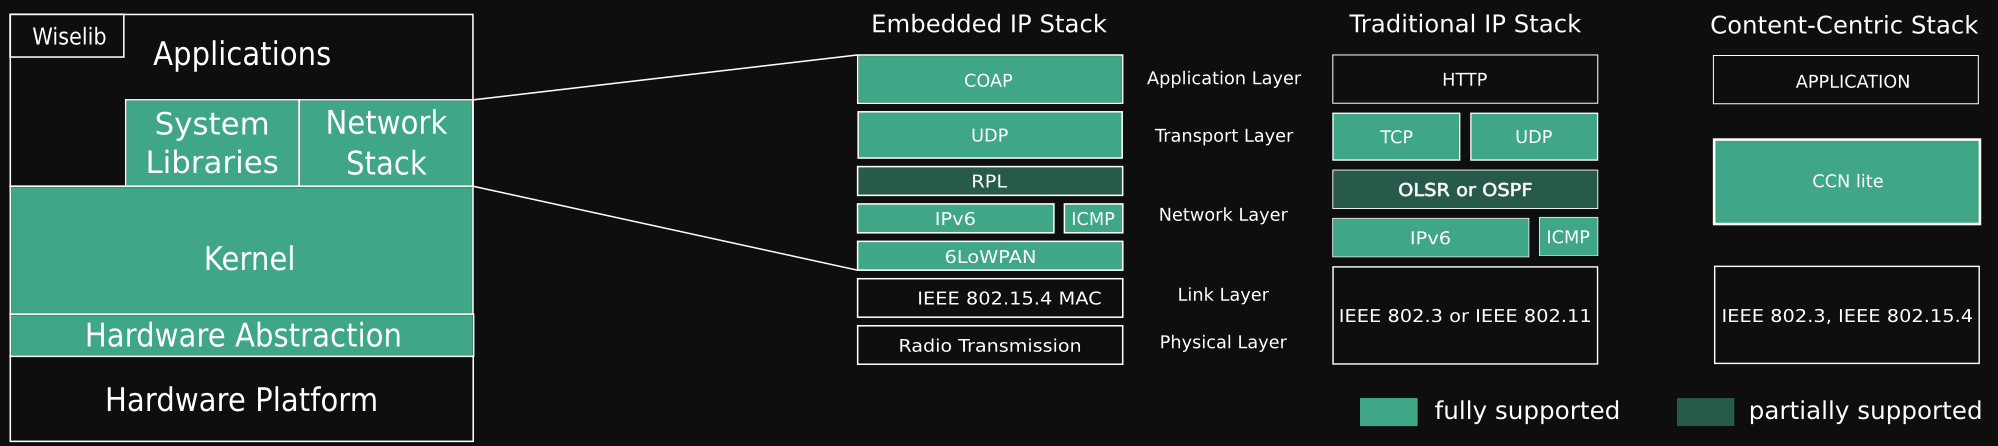
\includegraphics[width=1.0\linewidth]{bilder/RIOT.png}
  	\caption{�bersicht �ber das RIOT}
  	\label{fig:components}
  \end{figure} 
  \vspace{5mm} 
   
 RIOT-Programme k�nnen in C und C++ geschrieben werden. Es ist im Gegensatz zu anderen kleinen Betriebssystemen wie TinyOS echtes Multithreading verf�gbar. F�r Linux und MacOS existieren native Portierungen, so dass Anwendungen auf dem Computer geschrieben und dann schnell auf echte Hardware portiert werden k�nnen, was das Debugging erleichtern soll. Dabei werden Standardwerkzeuge wie GNU Compiler Collection (GCC), GNU Debugger benutzt.[3] Aufgrund der Herkunft als Betriebssystem f�r Sensornetzwerke bei der Feuerwehr ist RIOT echtzeitf�hig. Teile des POSIX-Standards sind implementiert.
 Der Quellcode liegt auf GitHub und wird von einer freien Entwickler-Community mitentwickelt.\cite{RIOTProjectDocumentation}
 
 \section{Aufbau}
 
 Dieser Abschnitt f�hrt Sie durch die Struktur von RIOT. Sobald Sie diese Struktur verstehen, verstehen Sie den RIOT-Code-Basis.
 
 \vspace{5mm} 
 \begin{figure}[h]
  \centering
  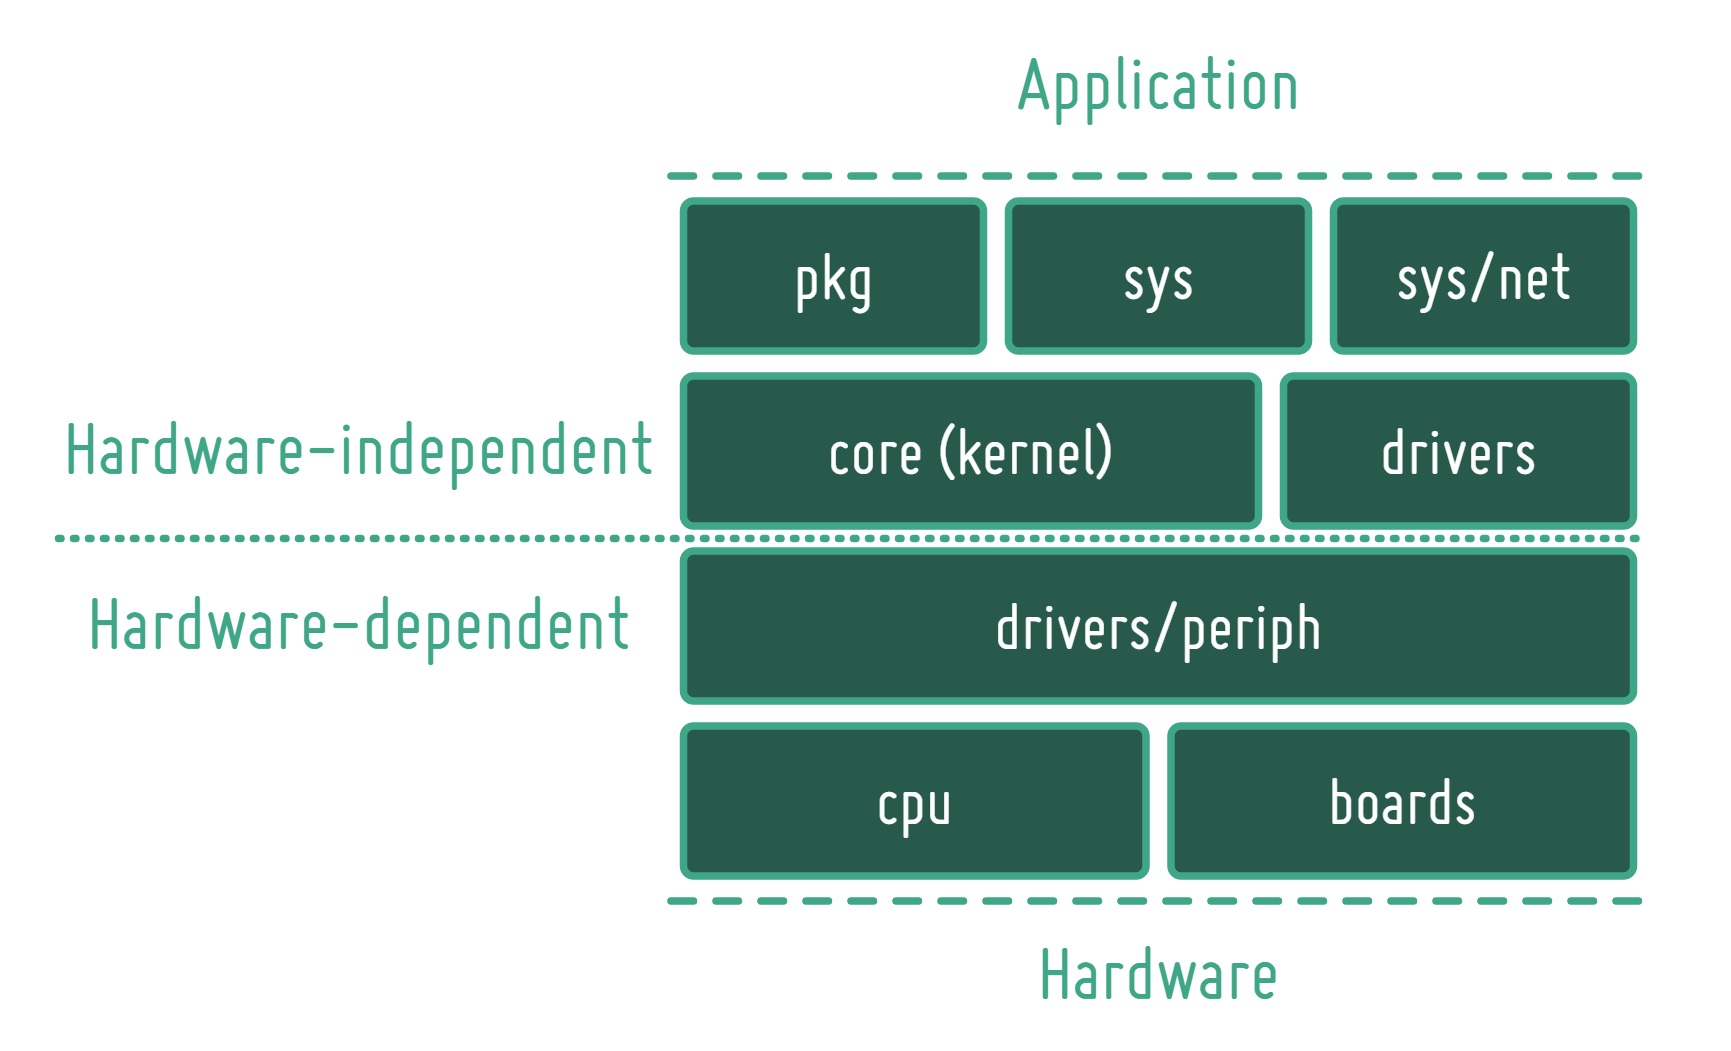
\includegraphics[width=0.8\linewidth]{bilder/RIOT.jpg}
  \caption{Struktur von RIOT}
  \label{fig:components}
 \end{figure}
 \vspace{10mm}

 
 Die Codebasis von RIOT ist in vier Gruppen eingeteilt.
  
 \begin{itemize}
   \item Der Kernel (Core)
   \item Plattformspezifischer Code (CPU)
   \item Ger�tetreiber (Drivers)
   \item Bibliotheken und Netzwerk-Code (sys; pkg)
 \end{itemize}
 \vspace{4mm}
  
  Dar�ber hinaus enth�lt RIOT eine Sammlung von Skripten f�r verschiedene Aufgaben, sowie eine vordefinierte Umgebung f�r die Erstellung dieser Dokumentation. Die Strukturgruppen werden auf die Verzeichnisstruktur von RIOT projiziert, wobei jede dieser Gruppen in einem oder zwei Verzeichnissen im Haupt-RIOT-Verzeichnis liegt. Die folgende Liste enth�lt eine detaillierte Beschreibung der einzelnen Verzeichnisse des RIOTs:
  
  
  \vspace{5mm}
  
  Core:
  
  Dieses Verzeichnis enth�lt den eigentlichen Kernel. Der Kernel besteht aus dem Scheduler, der Interprozess-Kommunikation (Messaging), dem Threading, der Threadsynchronisation und den unterst�tzenden Datenstrukturen und Typdefinitionen.
  
  \vspace{5mm}
  
  Board:
  
  Der plattformabh�ngige Code ist in zwei logische Elemente CPU und Board unterteilt. Eine Board hat genau eine CPU, w�hrend eine CPU Teil von vielen Boards sein kann. Der CPU-Teil enth�lt alle generischen, CPU-spezifischen Code.
  
  Der Board-Teil enth�lt die spezifische Konfiguration f�r die darin enthaltene CPU. Diese Konfiguration umfasst haupts�chlich die Peripheriekonfiguration und Pin-Mapping, die Konfiguration von On-Board-Ger�ten und die Taktkonfiguration der CPU. Zus�tzlich zu den Quell- und Header-Dateien, die f�r jedes Board ben�tigt werden, kann dieses Verzeichnis zus�tzlich einige Skript- und Konfigurationsdateien enthalten, die f�r die Anbindung an die Boards ben�tigt werden. 
  
  \vspace{5mm}
  
  CPU:
  
  F�r jede unterst�tzte CPU enth�lt dieses Verzeichnis ein Unterverzeichnis mit dem Namen der CPU. Diese Verzeichnisse enthalten dann alle CPU-spezifischen Konfigurationen, wie Implementierungen des Energiemanagements (LPM), Interrupt-Handler und Vektoren, Startupcode und Taktinitialisierungscode. F�r die meisten CPUs finden Sie auch die Linkerskripte im Unterverzeichnis.
  
  Im Periph-Unterverzeichnis jeder CPU finden Sie die Implementierungen der Peripherie-Treiber wie SPI, UART, GPIO, etc. Viele CPUs teilen einen bestimmten Code, z.B. alle ARM Cortex-M-basierten CPUs verwenden denselben Code f�r den Taskwechsel und den Interrupthandler. Dieser freigegebene Code hat ein eigenes Verzeichnis.
  
  \vspace{5mm}
  
  Drivers:
  
  Dieses Verzeichnis enth�lt die Treiber f�r externe Ger�te wie Netzwerkschnittstellen, Sensoren und Aktoren. Jeder Ger�tetreiber wird in ein eigenes Unterverzeichnis mit dem Namen des Ger�ts eingef�gt.
  
  Alle Ger�tetreiber des RIOT basieren auf der peripheren Treiber-API z.B. SPI, GPIO und anderen RIOT-Modulen wie dem xtimer. Auf diese Weise sind die Treiber v�llig plattformunabh�ngig.
  
  \vspace{5mm}
  
  Sys /net:
  
  RIOT folgt dem Mikrokern-Design-Paradigma, wo alles ein Modul sein soll. Alle diese Module, die nicht Teil der Hardware-Abstraktion oder Ger�tetreiber sind, k�nnen in diesem Verzeichnis gefunden werden. Die Bibliotheken umfassen Datenstrukturen, Kryptobibliotheken, Hight-level APIs und Speicherverwaltung. 

  Das Unterverzeichnis sys / net muss explizit erw�hnt werden, da hier der gesamte Netzwerkcode im RIOT liegt. Hier finden Sie die Netzwerk-Stack-Implementierungen z.B. den GNRC-Stack.
  
  \vspace{5mm}
  
  Pkg:
  
  RIOT unterst�tzt mehrere externe Bibliotheken z.B. OpenWSN, Microcoap. Die exteren Bibliotheken werden als benutzerdefinierte Makefiles ausgeliefert. Die Bibliothek l�dt optional eine Anzahl von Patches herunter, damit RIOT funktioniert. Diese Makefiles und Patches finden Sie im pkg-Verzeichnis.\cite{RIOTProjectDocumentation}
  
   \vspace{60mm}
  
 \section{Unterst�tzung}
 
  Momentan unterst�tzt der RIOT-Kernel gem�ss Angaben auf der Projektseite \cite{RIOTProjectDocumentation} Prozessoren der Architekturen ARM. Somit  kann es sowohl auf einem System-Emulator wie z.B. Qemu kompiliert werden oder auf einer unterst�tzten Hardware. Folgende Hardware-Hersteller wurden zum Zeitpunkt unserer Projektarbeit unterst�tz:

   
   \begin{center}
   	\begin{tabular}{ | l |}
   		\hline
   		\textbf{Hersteller} 	\\ \hline
   		Arduino		I 			\\ \hline
   		ARM architecture 		\\ \hline
   		Atmel 					\\ \hline
   		Freescale				\\ \hline
   		IoT-LAB					\\ \hline	
   		MSB						\\ \hline	
   		Nordic Semiconductor 	\\ \hline
   		Nucleo					\\ \hline
   		NXP						\\ \hline
   		PIC microcontroller		\\ \hline
   		STMicroelectronics		\\ \hline
   		Texas Instruments		\\ \hline
   	\end{tabular}
   \end{center}
   
 \vspace{4mm}
   
 Zur Kommunikation unterst�tzt das RIOT-Betriebssystem eine Vielzahl an Kommunikations-Protokolle. Da der Fokus auf das Internet der Dinge gelegt wurde, wurden auch die entsprechenden Protokolle zuerst implementiert. 
    
 Folgende Tabelle zeigt die Kommunikationsm�glichkeiten sowohl die vom Betriebssystem unterst�tzte Hardwarekomponenten wie auch die unterst�tzten Protokolle:
    
    
 \begin{center}
  \begin{tabular}{ | l | l |}
		\hline
		\textbf{Protokoll} 		& \textbf{Hardwarekomponente} \\ \hline
		Bluetooth 4.0 			& ADC 			\\ \hline
		CoAP / CSMA / CA		& Ethernet		\\ \hline
		IPv4 / IPv6				& Flash / RAM 	\\ \hline
		IEEE 802.15.4 		 	& GPIO			\\ \hline
		NTP / UNTP				& SPI			\\ \hline
		UDP / UHCP				& UART			\\ \hline
		6LoWPAN 				& 				\\ \hline
		Radios					& 				\\ \hline
		Wi-Fi					& 				\\ \hline
   \end{tabular}
  \end{center}




 % !TeX encoding = ISO-8859-1
 \chapter{Contiki-Overview}
 \label{chap:overview}
 
 \section{�bersicht �ber Contiki}
 
  Contiki ist ein Open-Source-Betriebssystem f�r das Internet der Dinge. Contiki verbindet winzige Low-Cost-, Low-Power-Mikrocontroller mit dem Internet. Contiki ist eine leistungsstarke Toolbox f�r den Aufbau komplexer drahtloser Systeme. Die Basis von Contiki und die meisten seiner Kernfunktionen, wie der Kernel, die meisten Bibliotheken, der uIP-Stack und der Rime-Stack wurdne von Adam Dunkels entwickelt.
  
  Contiki bietet einen einfachen ereignisgesteuerten Betriebssystemkern mit sogenannten Protothreads, optionalem Multiprogramming, Interprozesskommunikation via Messagepassing durch Events, eine dynamische Prozessstruktur mit Unterst�tzung f�r das Laden von Programmen, nativen TCP/IP-Support �ber den uIP TCP/IP-Stack und eine grafische Benutzerschnittstelle, welche direkt auf einem Bildschirm oder als virtuelle Anzeige �ber Telnet oder VNC genutzt werden kann. Der Speicherbedraf betr�gt nur wenige Kilobyte und kann f�r extrem eingeschr�nkte Systeme bei Bedarf bis auf einige dutzend Bytes reduziert werden. Inzwischen unterst�tzt Contiki auch IPv6.
  An Anwendungsprogrammen bietet das System einen Webbrowser, einen Web-Server, einen Telnet-Server und vieles mehr.
   
  \begin{figure}[h]
   \centering
   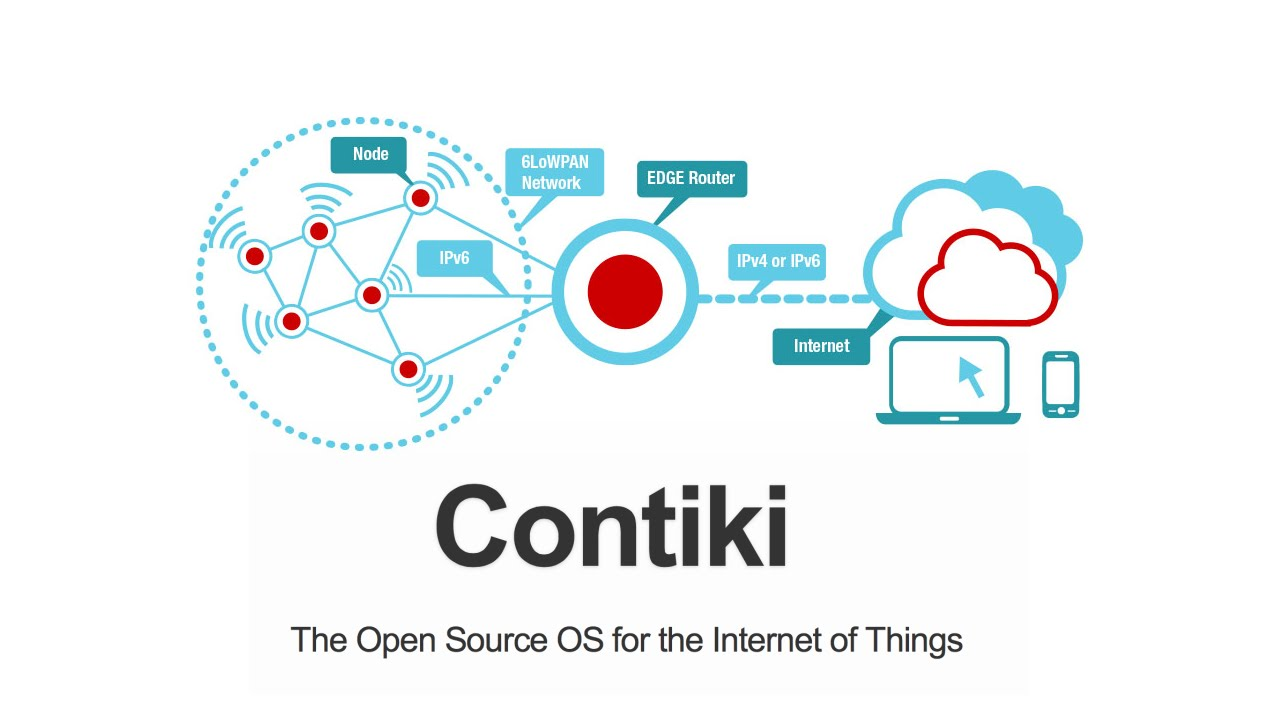
\includegraphics[width=1.0\linewidth]{bilder/Contiki.jpg}
   \caption{�bersicht �ber das Contiki OS}
   \label{fig:components}
  \end{figure}
  
  \vspace{5mm}
  
  Wegen seiner Portabilit�t wurde und wird dieses System an viele Computer angepasst, wie Atari 8-bit-Rechner oder Apple II. Eine der am aktivsten entwickelten Portierungen ist die auf den C64, die sogar eine ebenfalls von Adam Dunkels entwickelte Ethernetanbindung unterst�tzt. PCs k�nnen Contiki ausf�hren und es gibt sogar eine Portierung f�r kleinere Spielekonsolen wie dem Game Boy.
  Daneben findet die Software Einsatz in der Middleware und den Sensoren des RUNES Projekts, Reconfigurable Ubiquitous Networked Embedded Systems.
 
  Der Contiki-Quellcode wird unter einer 3-Klausel BSD-Lizenz ver�ffentlicht. Unter dieser Lizenz kann Contiki frei in kommerziellen und nicht-kommerziellen Systemen verwendet werden, solange das Copyright-Header in den Quellcodedateien beibehalten wird.
  Das Copyright f�r den Contiki-Quellcode liegt im Besitz der Personen oder Organisationen, die es zu Contiki beigetragen haben, aber jeder hat es unter denselben Bedingungen der BSD-Lizenzbestimmungen mitgeteilt.\cite{ContikiProjectDocumentation}
  
 
 \section{Ziele}
 
  Contiki entstand aus dem Wunsch von Adam Dunkels, unerwartete Dinge mit dem Internet zu verbinden. 2001 wurde der Open-Source-UIP-Stack als kleinerer Cousin zu lwIP entwickelt und verbreitete sich rasch �ber die Embedded World. Aber uIP war nicht nur in zahlreichen tief eingebetteten Systemen, sondern auch im Internet der Dinge verwendet. 2003 folgte Contiki.
  Im Jahr 2004 wurde das Konzept der Protothreads, das nun die Grundlage f�r die Prozesse von Contiki bildet, in Contiki eingef�hrt. Fr�he Versionen von Cooja und dem Rime-Stack wurden 2007 mit Contiki 2.0 hinzugef�gt. Power-Profiling wurde 2007 entwickelt. Instant Contiki und das Coffee-Dateisystem wurden Anfang 2008 eingef�hrt. Sp�ter f�hrte Cisco den vollst�ndig zertifizierten IPv6-Stack zu Contiki ein.
  2009 und 2010 wurden viele neue Plattformen zu Contiki hinzugef�gt und neue Low-Power-Mechanismen entwickelt. 2011 wurden zwei wichtige Mechanismen hinzugef�gt: ContikiRPL, f�r IPv6-Routing und ContikiMAC f�r schl�frige Router.
  Im Jahr 2012 wurde Thingsquare gegr�ndet, um Contiki in die Cloud zu bringen.\cite{ContikiProjectDocumentation}
  
  
 \section{Aufbau}
 
 Contiki bietet leistungsstarke Low-Power-Internet-Kommunikation. Contiki unterst�tzt vollst�ndig Standard IPv6 und IPv4, zusammen mit den j�ngsten Low-Power-Wireless-Standards: 6lowpan, RPL, CoAP. Mit Contiki's ContikiMAC und schl�frigen Routern k�nnen sogar drahtlose Router batteriebetrieben werden.\cite{ContikiProjectDocumentation}
 
   \begin{figure}[h]
   	\centering
   	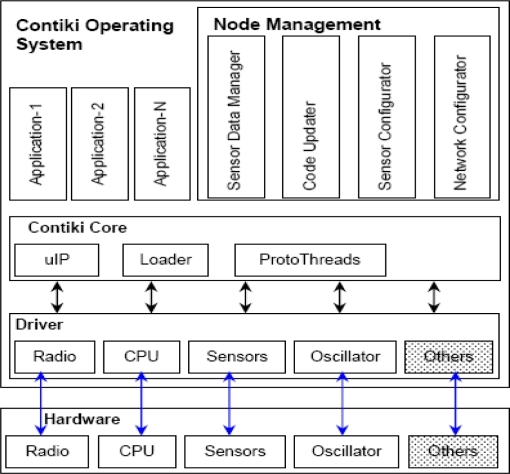
\includegraphics[width=0.7\linewidth]{bilder/Contiki.png}
   	\caption{Struktur des Contiki OS}
   	\label{fig:components}
   \end{figure}

  \vspace{5mm}
 
 Memory Allocation:
 
 Contiki ist f�r kleine Systeme mit nur wenigen Kilobyte Speicherplatz ausgelegt. Contiki ist daher hochspeicherf�hig und stellt einen Satz von Mechanismen f�r die Speicherzuteilung bereit: Speicherblockzuteilung Membran, einen verwalteten Speicherzuweiser mmem sowie den Standard-C-Speicherzuweiser malloc.
 
  \vspace{5mm}
 
 Power Awareness:
 
 Contiki ist f�r den Betrieb in extrem energiesparenden Systemen ausgelegt: Systeme, die m�glicherweise Jahre an einem Paar AA-Batterien betrieben werden m�ssen. Um die Entwicklung von energiesparenden Systemen zu unterst�tzen, bietet Contiki Mechanismen zur Sch�tzung des Energieverbrauchs des Systems und zum Verst�ndnis, wo die Energie verbraucht wurde.
 
  \vspace{5mm}
 
 6lowpan, RPL, CoAP:
 
 Contiki unterst�tzt die k�rzlich standardisierten IETF-Protokolle f�r Low-Power IPv6-Netzwerke, einschlie�lich der 6lowpan-Adaptionsschicht, des RPL-IPv6-Multi-Hop-Routingprotokolls und des CoAP RESTful-Anwendungsschichtprotokolls.
 
 \vspace{5mm}
 
 Dynamic Module Loading:
 
 Contiki unterst�tzt dynamisches Laden und Verkn�pfen von Modulen zur Laufzeit. Dies ist n�tzlich bei Anwendungen, bei denen das Verhalten nach der Implementierung ge�ndert werden soll. Der Contiki-Modul-Loader kann Standard-ELF-Dateien laden, verlagern und verkn�pfen, die wahlweise von den Debugging-Symbolen entfernt werden k�nnen, um deren Gr��e beizubehalten.
 
  \vspace{5mm}
 
 Memory Footprint:
 
 Contiki ist entworfen worden, um in kleinen Mengen des Ged�chtnisses laufen zu lassen. Ein typisches System mit voller IPv6-Vernetzung mit schl�frigen Routern und RPL-Routing ben�tigt weniger als 10 k RAM und 30 k ROM.
 

 \section{Unterst�tzung}

 Momentan unterst�tzt der Contiki-Kernel gem�ss Angaben auf der Projektseite \cite{ContikiProjectDocumentation} Prozessoren der Architekturen ARM. Folgende Hardware-Hersteller wurde zum Zeitpunkt unserer Projektarbeit unterst�tz:
 
\begin{center}
  \begin{tabular}{ | l |}
	\hline
	\textbf{ARM} 				\\ \hline
	Atmel AVR			 		\\ \hline
	Microchip pic32mx795f512l 	\\ \hline
	Microchip pic32mx795f512l	\\ \hline
	nRF52832 					\\ \hline
	RL78						\\ \hline
	TI CC2538					\\ \hline	
	TI CC2538					\\ \hline	
	TI MSP430 					\\ \hline
	\hline
 \end{tabular}
\end{center}
\vspace{4mm}

 Zur Kommunikation unterst�tzt das Contiki-Betreibssystem eine Vielzahl an Kommunitations-Protokolle. Da der Fokus auf das Internet der Dinge gelegt wurde, wurden auch die entsprechenden Protokolle zuerst implementiert. 
 
 Folgende Tabelle zeigt die Kommunikationsm�glichkeiten sowohl die vom Betriebssystem unterst�tzte Hardwarekomponenten wie auch die unterst�tzten Protokolle:
 
 
 \begin{center}
 	\begin{tabular}{ | l | l |}
 		\hline
 		\textbf{Protokoll} 		& \textbf{Hardwarekomponente} \\ \hline
 		Bluetooth 4.0 			& GPIO 		\\ \hline
 		CoAP					& I2C		\\ \hline
 		HTTP					& SPI		\\ \hline
 		IPv4 / IPv6				& UART	 	\\ \hline
 		IEEE 802.15.4 		 	& 			\\ \hline
 		TCP						& 			\\ \hline
 		UDP / UHCP				& 			\\ \hline
 		6LoWPAN 				& 			\\ \hline
 		Radios					& 			\\ \hline
 		RPL						& 			\\ \hline
 		Wi-Fi					& 			\\ \hline
 		\hline
 	\end{tabular}
 \end{center}
 
 \vspace{5mm}
 

 
 
 

 

 

 
 

 

 % !TeX encoding = ISO-8859-1
 \chapter{NuttX Real-Overview}
 \label{chap:overview}
 
 \section{�bersicht �ber NuttX Real}
 
 NuttX ist ein Echtzeitbetriebssystem (RTOS) mit einem Schwerpunkt auf Normenkonformit�t und geringem Platzbedarf. Skalierbar von 8-Bit- bis 32-Bit-Mikrocontroller-Umgebungen sind die prim�ren Normen in NuttX die Posix- und ANSI-Standards. Zus�tzliche Standard-APIs von Unix und anderen g�ngigen RTOS, wie VxWorks, werden f�r die Funktionalit�t, die unter diesen Standards nicht verf�gbar ist, oder f�r Funktionalit�ten, die f�r tief eingebettete Umgebungen wie zum Beispiel ''fork'' nicht geeignet sind, �bernommen. NuttX wurde zuerst 2007 von Gregory Nutt unter der permissiven BSD Lizenz ver�ffentlicht. NuttX, wie bei vielen RTOS, ist eine Sammlung von verschiedenen Funktionen geb�ndelt als Bibliothek. Es wird nicht ausgef�hrt ausser wenn entweder:\cite{NuttXProjectDocumentation}
 
  \begin{itemize}
  	\item Die Anwendung den NuttX-Bibliothekscode aufruft
  	\item Ein Interrupt auftritt

  \end{itemize}  
  
 NuttX implementieren ein virtuelles Dateisystem ''VFS'', das verwendet werden kann, um mit einer Anzahl von verschiedene  Entities  Schnittstellen   �ber die standardm�ssigen open(), close(), read(), write(), etc. zu kommunizieren. Wie andere VFSs unterst�tzt das NuttX VFS Dateien, Verzeichnisse, Ger�tetreiber. Auch wie bei anderen VFSs unterst�tzt das  NuttX-Dateisystem psuedo-Dateisysteme. Das NuttX-Root-Dateisystem ist immer ein Pseudo-Dateisystem. Das ist genau das Gegenteil von Linux. Mit Linux muss das Root-Dateisystem immer ein physikalisches Block-Device sein. Bei NuttX ist das Root-Dateisystem immer ein Pseudofile System, das keinen zugrunde liegenden Blocktreiber oder physikalisches Ger�t ben�tigt. Diese Anordnung macht das Leben viel einfacher f�r die kleine eingebettete Welt. NuttX interagiert mit Ger�ten �ber Ger�tetreiber - das hei�t �ber Software wird die Hardware steuert. Wenn eine Task einen pthread erzeugt, teilen er die Umgebungsvariablen, Dateideskriptoren, Sockets und Streams. Diese Task-Ressourcen werden als Referenz gez�hlt und bleiben so lange bestehen, wie Thread in der Task-Gruppe aktiv ist:\cite{NuttXProjectPDF}
    
 \begin{itemize}
  \item Umgebungsvariablen, ist die Sammlung von variablen Zuordnungen: ''VARIABLE = VALUE'' 	
  \item Ein Dateideskriptor ist eine aufgabenbezogene Zahl, die eine offene Ressource darstellt, Datei oder einen Ger�tetreiber
  \item Ein Socket-Deskriptor ist wie ein Dateideskriptor, aber die offene Ressource ist in diesem Fall ein Netzwerk-Buchse
  \item Streams wickeln Dateideskriptoren oder Sockets ein und bieten einen neuen Satz von Schnittstellenfunktionen f�r den Umgang mit der Standard-C Funktionen an  	
 \end{itemize}
   
 
 \section{Ziele}
 
 Es gibt einige RTOS-Funktionen, die durch interne Threads implementiert werden.
 Um ein Echtzeit-OS zu sein, muss ein RTOS ''SCHED FIFO'' unterst�tzen. Das hei�t, strenge Priorit�t Scheduling. Eines Scheduler: Diese Logik, die steuert, wenn Tasks oder Threads ausgef�hrt werden. Der Scheduler bestimmt, was eine Task oder ein Thread ist. In NuttX ist ein Thread eine beliebige steuerbare Sequenz der Befehlsausf�hrung, die einen eigenen Stack hat. Jede Aufgabe wird durch eine Datenstruktur dargestellt, die als Task-Steuerblock oder TCB bezeichnet wird. Diese TCBs werden in Listen aufbewahrt. Der Zustand einer Task wird im Feld ''Task State'' angezeigt. Die meisten dieser Listen sind priorisier. So dass eine gemeinsame Listenhandhabungslogik verwendet werden kann. Threads, die vom Betriebssystem verwaltet werden. Ein Prozess ist mehr als ein Thread, wie wir bisher diskutiert haben. Ein Prozess ist eine gesch�tzte Umgebung, die einen oder mehrere Threads hostet. Unter Umgebung verstehen wir den Satz von Ressourcen von der OS.

 Um den Adressraum des Prozesses zu implementieren, muss die CPU eine Speicherverwaltungseinheit  MMU unterst�tzen. Allerdings wurde NuttX entworfen auch mit beschr�nkten Ressourcen zufunktionieren. Diese CPUs haben selten eine MMU und k�nnen daher Prozesse niemals unterst�tzen. So unterst�tzt NuttX keine Prozesse. NuttX arbeitet nur in einem flachen Adressraum, um Befehls- und Datencaches zu steuern und gesch�tzte Speicherbereiche zu unterst�tzen. Die dem TCB am Anfang der readytorun-Liste zugeordnet ist. NuttX unterst�tzt eine weitere Echtzeit-Planungsrichtlinie: ''SCHED RR''. Die RR steht f�r Roundrobin, dies wird manchmal als Round-Robin-Scheduling bezeichnet. In diesem Fall unterst�tzt NuttX das Timelicing. Jede Aufgabe wird nicht nur durch eine TCB, sondern auch durch eine numerische Task-ID dargestellt. Bei einem TCB kann das RTOS die Task-ID finden. Sie sind also funktional gleichwertig.\cite{NuttXProjectPDF}
 

 \section{Aubau}
 
  Auf der h�chsten Ebene kann die NuttX-Initialisierungssequenz in drei Phasen dargestellt werden:
  
   \begin{itemize}
   	\item Die hardware-spezifische Einschalt-Reset-Initialisierung	
   	\item NuttX RTOS Initialisierung
   	\item Anwendungsinitialisierung
  	
   \end{itemize}

  Diese Initialisierungssequenz ist wirklich ganz einfach, weil das System im Single-Thread-Modus l�uft. Kurz vor dem Starten der Anwendung geht das System in den Multi-Thread-Modus. Die Software beginnt mit der Ausf�hrung, sobald der Prozessor ein Power-on, oder ein Reset, oder Watchdog Signal erh�t. Die Software, die ausgef�hrt wird, ist f�r die jeweilige CPU eindeutig. Architektur und ist kein gemeinsamer Bestandteil von NuttX. Die Art der Dinge, die von der Architektur-spezifische Reset-Handling beinhaltet:\cite{NuttXProjectPDF}
  
     \begin{itemize}
     	\item Setzen des Prozessors in seinen Betriebszustand. Setzen der CPU-Modi und Initialisierung von Co-Prozessoren
     	\item Einstellen der Taktung, so dass die Software und Peripherie wie erwartet funktionieren und einrichten des C-Stack-Zeigers
     	\item Speicher initialisieren und Starten von NuttX	
     \end{itemize}

 \section{Unterst�tzung}
 
 Momentan unterst�tzt der NuttX-Kernel gem�ss Angaben auf der Projektseite \cite{NuttXProjectDocumentation} Prozessoren der Architekturen ARM. Folgende Hardware wurde zum Zeitpunkt unserer Projektarbeit unterst�tz:
 
 
 \begin{center}
 	\begin{tabular}{ | l |}
 		\hline
 		\textbf{Hersteller} 				\\ \hline
 		ARM7TDMI 							\\ \hline
 		ARM920T 							\\ \hline
 		ARM926EJS 							\\ \hline
 		ARM Cortex-A5						\\ \hline	
 		ARM Cortex-A8						\\ \hline
 		ARM Cortex-R4/R4F					\\ \hline
 		ARM Cortex-M0 						\\ \hline
 		ARM Cortex-M3 						\\ \hline
 		ARM Cortex-M4 						\\ \hline
 		ARM Cortex-M7 						\\ \hline
 		Atmel 8-bit AVR (AT90USB, ATmega)	\\ \hline
 		AVR32								\\ \hline
 		Freescale M68HCS12					\\ \hline
 		Intel X86							\\ \hline
 		MicroChip PIC32MX (MIPS32 24Kc)		\\ \hline
 		MicroChip PIC32MZ (MIPS32 M14k)		\\ \hline
 		Renesas/Hitachi SuperH				\\ \hline
	 	Renesas M16C/26						\\ \hline
 		Zilog Z16F ZNeo						\\ \hline
 		Zilog eZ80 Acclaim					\\ \hline
 		Zilog Z8Encore						\\ \hline
 		Zilog Z80 							\\ \hline
 		\hline
 	\end{tabular}
 \end{center}
 
 \vspace{4mm}
 
  Zur Kommunikation unterst�tzt das NuttX-Betreibssystem eine Vielzahl an Kommunikations-Protokolle. Da der Fokus auf das Internet der Dinge gelegt wurde, wurden auch die entsprechenden Protokolle zuerst implementiert. 
  
  Folgende Tabelle zeigt die Kommunikationsm�glichkeiten sowohl die vom Betriebssystem unterst�tzte Hardwarekomponenten wie auch die unterst�tzten Protokolle:
  
  
  \begin{center}
  	\begin{tabular}{ | l | l |}
  		\hline
  		\textbf{Protokoll} 		& \textbf{Hardwarekomponente} \\ \hline
  		DHCP 						& ADC 		\\ \hline
  		HTTP						& CAN		\\ \hline
	  	ICMP /  ICMPv6 / ICMPv2		& GPIO		\\ \hline
  		IPv4 / IPv6					& I2C	 	\\ \hline
  		TCP	/ IP					& PWM			\\ \hline
  		NFR							& SPI			\\ \hline
  		UDP / APR					& UART			\\ \hline
  		6LoWPAN 					& USB			\\ \hline
  		\hline
  	\end{tabular}
  \end{center}
  

 

% !TeX encoding = ISO-8859-1
\chapter{nRF52DK}
\label{chap:nrf52dk}

\begin{figure}[h]
	\centering
	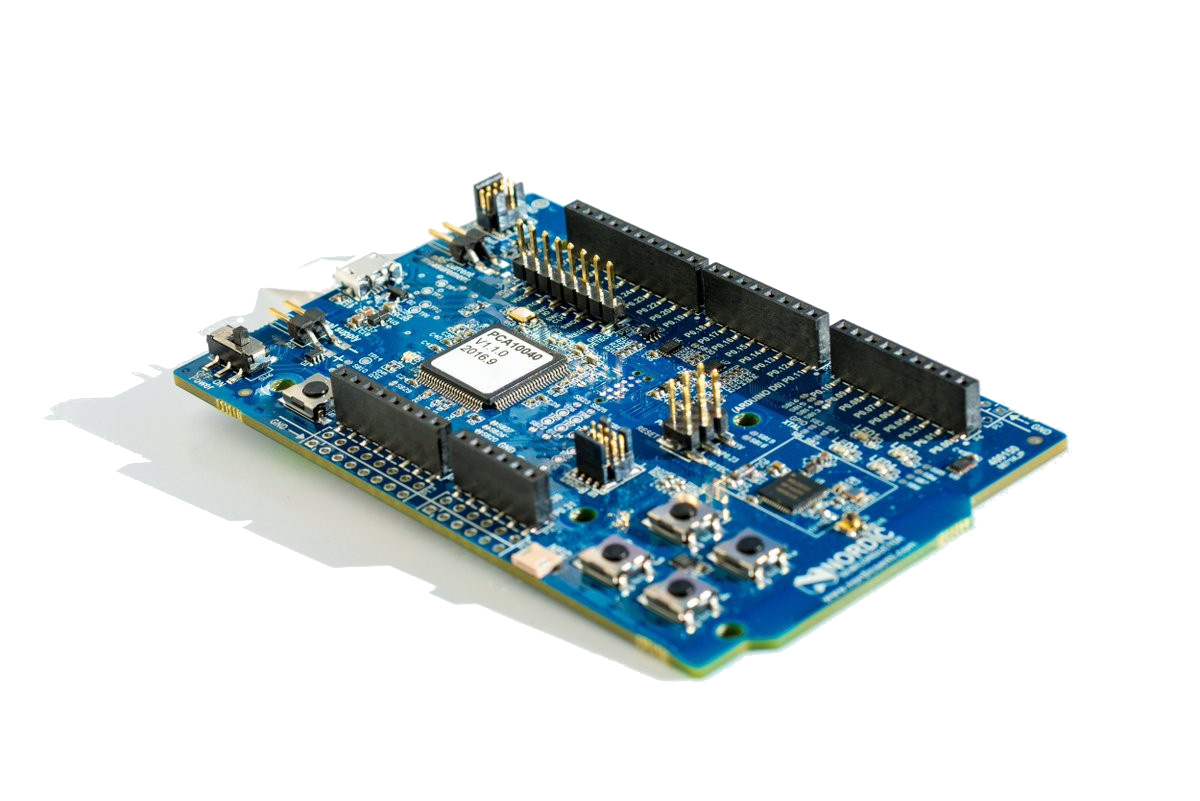
\includegraphics[width=1.0\linewidth]{bilder/nrf52_board.jpg}
	\caption{Das nRF52 Development Kit}
	\label{fig:devkit}
\end{figure}

Das nRF52 DK ist eine single-Board Entwicklungsplatform welche f�r die Verwendung von \ac{BLE}, ANT, und propriet�ren 2.4GHz Protokollen ausgelegt ist. Herzst�ck des Kits ist das nRF52832 \ac{SoC}.

Die Header sind kompatibel mit allen Arduino Shields des Revisionsstandards 3 was das Kit enorm erweiterbar macht. Weiter besteht die M�glichkeit eine mitgelieferte NFC-Antenne anzuschliessen um NFC-Tags zu lesen. Alle GPIOs sind via Header herausgef�hrt. Zus�tzlich verf�gt das Board �ber 4 LEDs und 4 Taster. 

\newpage

\section{Technische �bersicht}

\begin{figure}[h]
	\centering
	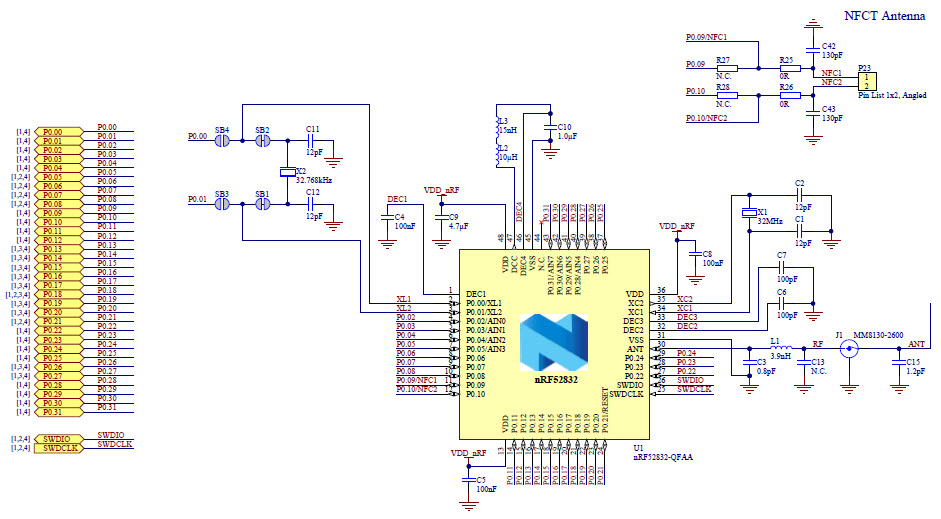
\includegraphics[width=1.0\linewidth]{bilder/nrf52_schematic.jpg}
	\caption{Schema des nRF52DKs aus der Dokumentation von Nordic entnommen}
	\label{fig:schematic}
\end{figure}

\section{Installation der GNU ARM Embedded Toolchain}

Um die Funktion aller Tools und der SDK zu gew�hrleisten, sollten folgende Installationen ausschliesslich in der hier beschriebenen Reihenfolge ausgef�hrt werden. Da sich die Installation unter Ubuntu und Arch Linux unterscheiden, sind im nachfolgenden beide Varianten dokumentiert. 

Um die Software auf dem Hostsystem f�r das nRF52DK kompilieren zu k�nnen, ben�tigen wir eine sogenannte crosscompiler-toolchain. F�r ARM basierte Controller ist hier die erste Wahl die gnu-arm-none-eabi Toolchain. Sie l�sst sich von folgender Seite beziehen:

\url{https://launchpad.net/gcc-arm-embedded/+download}

Es gilt darauf zu achten, die neueste Version zu verwenden und sich zu notieren, welche Version heruntergeladen wurde, da diese sp�ter im Makefile angegeben werden muss. Die Software sollte im Verzeichnis /opt installiert werden. Die Binaries sollten mit den n�tigen Rechten ausgestattet werden. Weiter empfiehlt es sich symbolische Links zu generieren, um die Programme systemweit sichtbar zu machen.

Die Befehle dazu lauten:

\begin{lstlisting}[style=BashInputStyle]
    tar -xf gcc-arm-none-eabi-linux.tar.bz2 /opt/gcc-arm-none-eabi-tools
    ln -s /opt/gcc-arm-none-eabi-tools/bin/* /usr/local/bin/
\end{lstlisting}

Wichtig: Unter Arch Linux sollte unbedingt die aktuellste Version im Community Repository verwendet werden. Die gew�nschte Software l�sst sich wie folgt installieren:

\begin{lstlisting}[style=BashInputStyle]
    pacman -S community/arm-none-eabi-binutils
    pacman -S community/arm-none-eabi-newlib
    pacman -S community/arm-none-eabi-gcc
    pacman -S community/arm-none-eabi-gdb
\end{lstlisting}


\section{Installation der nordic SDK}

Nordic Semiconductor verf�gt �ber ein Software Archiv von welchem alle ben�tigte Software bezogen werden kann. Das Archiv befindet sich unter folgendem Link:

\url{https://www.nordicsemi.com/eng/Products/Bluetooth-low-energy/nRF52-DK#Downloads}

Um mit dem nRF52 Entwicklungskit arbeiten zu k�nnen, ben�tigen wir folgende Softwarepakete:

\begin{enumerate}
    \item nRF5 SDK Zip File
    \item nRF5x-Command-Line-Tools-Linux64
\end{enumerate}

Im ersten Paket befinden sich alle Files, welche zur Entwicklung von Software auf dem nRF52dk notwendig sind. Darunter Makefiles, Linkerskripte und auch Beispielcode.
Im zweiten Paket befinden sich die Command-Line-Tools, welche es uns erm�glichen �ber die Kommandozeile mit dem nRF52 Entwicklungskit zu kommunizieren. Das wichtigste Tool ist nrfjprog, welches kompilierte Programme auf das Board hochladen kann.

Die SDK sowie die Command-Line-Tools sollten auf dem System unter dem Ordner /opt installiert werden und mit den n�tigen Berechtigungen versehen werden. Ebenfalls sollten die Programme in einen Ordner gelinkt werden, welcher im Systempfad angegeben ist.

Die Befehle dazu lauten:
\begin{lstlisting}[style=BashInputStyle]
    tar -xf nRF5x-Command-Line-Tools-Linux64.tar /opt/
    ln -s /opt/nrfjprog/nrfjprog /usr/bin/nrfjprog
    ln -s /opt/mergehex/mergehex /usr/bin/mergehex
\end{lstlisting}

Unter Arch Linux lassen sich die Command Line Tools auch �ber das Arch User Repository beziehen. Dazu kann man den Pacman Wrapper ''yaourt'' verwenden:

\begin{lstlisting}[style=BashInputStyle]
    yaourt -S aur/nrf5x-command-line-tools 
\end{lstlisting}

\section{Installation des SEGGER JLink Debuggers}

Die Software von SEGGER, welche f�rs Debuggen gebraucht wird, findet man unter folgendem Link:

\url{https://www.segger.com/downloads/jlink}

Das Paket ''J-Link Software and Documentation Pack'' enth�lt verschiedene Programme. Die Wichtigsten davon sind der JLinkCommander und der JLinkGDBServer. �ber den Commander l�sst sich die CPU des nRF52 vollst�ndig via JTAG oder SWD Schnittstelle kontrollieren. Der JLinkGDBServer stellt auf dem Localhost einen Socket unter Port 2331 zur Verf�gung, auf welchen man sich mit GDB verbinden kann.

Die JLink Toolchain sollte auf dem System unter dem Ordner /opt installiert werden und mit den n�tigen Berechtigungen versehen werden. Die Programme sollten mittels symbolischen Links in einen Ordner gelinkt werden, welcher im Systempfad angegeben ist.

\begin{lstlisting}[style=BashInputStyle]
    mkdir /opt/SEGGER/JLink
    tar -xzf JLink_Linux_{VERSION}.tar.gz /opt/SEGGER/JLink
    ln -s /opt/SEGGER/JLink/JLinkExe /usr/bin/JLinkExe
    ln -s /opt/SEGGER/JLink/JLinkGDBServer /usr/bin/JLinkGDBServer
\end{lstlisting}

SEGGER bietet auch ein Debianpaket an. Dieses kann auf Systemen, welche �ber den Paketmanager DPKG verf�gen mittels \verb|dpkg -i JLink_linux.deb| installiert werden. Dadurch entf�llt obiger Installationsaufwand.\newline

Unter ArchLinux l�sst sich die Software auch aus dem Arch-User-Repository installieren, der Befehl dazu lautet:
\begin{lstlisting}[style=BashInputStyle]
    yaourt -S aur/jlink-software-and-documentation
\end{lstlisting}

\section{Verwendung des JLinkGDBServers}

Der folgende Befehl beschreibt das Starten des GDBJLinkServers von SEGGER. 

\begin{lstlisting}[style=BashInputStyle]
    JLinkGDBServer -Device nRF52832_xxAA -If SWD -Speed 4000 -Autoconnect 1
\end{lstlisting}

Der Server startet einen lokalen Socket und ist unter Port 1234 erreichbar.
Nachdem \ac{GDB} gestartet wurde, l�sst sich �ber folgenden Befehl eine Verbindung mit dem Server herstellen:

\textbf{(gdb) target remote localhost:1234}

Alternativ kann auch eine Konfigurationsdatei f�r GDB angelegt werden. Dazu erstellt man im Home-Verzeichnis eine Datei mit dem Namen .gdbinit. Um automatisch auf den lokalen Server zu verbinden ist lediglich die obere Zeile hinzuf�gen. 

\section{Verwendung von nrfjprog}

Nrfjprog ist Teil der Propriet�ren Softwarewerkzeuge der SDK von Nordic. Es unterst�tzt das Flashen von Hex-Binarys �ber SWD oder JTAG. Der Funktionsumfang ist sehr gross, daher sei an dieser Stelle auch noch aufs Helpfile verwiesen.

Um eine bereits kompilierte Beispielapplikation auf das nrf52 Board zu laden sind folgende Befehle in dieser Reihenfolge auszuf�hren.

\begin{lstlisting}[style=BashInputStyle]
    nrfjprog --eraseall -f nrf52
    nrfjprog --program outdir/nrf52_pca10040/zephyr.hex -f nrf52
    nrfjprog --reset -f nrf52
\end{lstlisting}

Zeile 1 l�scht den aktuellen Inhalt des Flashspeichers auf dem SoC.\newline
Zeile 2 flasht ein neues Binary in den Flashspeicher des SoC.\newline
Zeile 3 Resetet den SoC, alternativ kann auch der Hardwarereset bet�tigt werden.\newline

% !TeX encoding = ISO-8859-1
\chapter{DemoApp}
\label{chap:demoapp}

\section{Technische �bersicht}
\section{Hardware Dokumentation}
\section{Software Dokumentation}
\section{Softwaretests}
% !TeX encoding = ISO-8859-1
\chapter{Fazit}
\label{chap:fazit}

\section{Vergleich Ist/Soll}

Wir sind mit dem erreichten Resultat zufrieden. Unsere Arbeit bietet einen horizontalen �berblick �ber das Zephyr-Betriebssystem. Ausserdem konnte ein detaillierter Beschrieb des Aufbaus und der Ziele des Betriebssystems erl�utert werden. Zudem wird ein �berblick �ber einige technische Details, wie z.B. Technologien, Protokolle und Anwendungen gew�hrt. Im Vergleich zu anderen Berichten, sofern diese schon vorliegen in diesem Bereich, konnten wir unser Ziel, eine umfassendere Zusammenfassung der wichtigsten Protokolle und Anwendungsprobleme bieten, damit Forscher und Anwendungsentwickler einen schnellen �berblick �ber die gew�nschten Funktionalit�ten erhalten. 

Ein weiteres Ziel das wir uns f�r die Projektarbeit gestellt haben ist die Entwicklung einer Demonstrationsapplikation f�r Zephyr, welche als Beispielprojekt f�r Neuentwicklungen dienen kann. Im Verlaufe der Projektarbeit musste das Pflichtenheft dieser Demoapp leider abgespeckt werden. Das Zephyr-OS war zur Zeit der Durchf�hrung der Projektarbeit noch unter aktiver Entwicklung. Auch die Unterst�tzung des nRF52 Development Kits beschr�nkte sich gr�sstenteils auf Bluetooth und Wireless. Die Dokumentation aller weiteren Funktionalit�ten f�r das Board war noch nicht vorhanden, was Entwicklungsarbeiten enorm erschwerte. Die Ursache ist damit zu begr�nden, dass das Board wegen der propriet�ren Toolchain vom Buildsystem noch nicht vollst�ndig unterst�tzt ist. Das bedeutet, dass zur Entwicklung Tools wie die Eclipse IDE nur beschr�nkt einsetzbar sind.
Im Rahmen der Projektarbeit haben wir daher ein Shellscript geschrieben welche die oben genannten Funktionalit�ten mit bringt. Eine Anpassung des Makefiles des Zephyr Build-Systems w�re w�nschenswert und w�rde den Support der Produktepalette von Nordic ganz sicher vorantreiben. Dies h�tte jedoch den von uns gesteckten Rahmen der Arbeit gesprengt, daher haben wir uns auf die Entwicklung des Shellscripts begrenzt.
Als Demonstrationsapplikation dient momentan das Eddystone Beacon Example des Zephyrprojektes. Das Beispielprogramm wurde jedoch f�rs nRF52 Board angepasst und in ein eigenes Projekt umgewandelt. Weiter entwickelten wir eine "Hello World" Applikation welche vom nrf52dk-zephyr-tool beim Anlegen eines neuen Projektes generiert wird. Diese Applikation zeigt die Verwendung der GPIOs des Boards. 
Die gesammelten Erfahrungen k�nnen in sp�teren Projekten der Berner Fachhochschule bestimmt gut gebraucht werden. Als Schlussbetrachtung kann gesagt werden, dass das Projekt eine gewisse Herausforderung war. Viele Teile des Zephyr-Projektes sind noch nicht Dokumentiert und es bedurfte bis zu einem gewissen Grad Reverse Engineering und Trial-And-Error um beispielsweise die richtigen Kernelkonfigurationen zu finden, damit die Software auf unserem Board l�uft. Nichtsdestotrotz war es ein sehr interessantes und abwechslungsreiches Projekt. 

Wir m�chten uns hiermit bei unserem Betreuer Herr Martin Aebersold f�r die gute Unterst�tzung bedanken.

\section{W�nschenswerte Erweiterungen}

W�nschenswert w�re sicher die Erweiterung des Makefiles um das nRF52 Board besser zu unterst�tzen. Weiter sollte man sich vertiefter mit der Entwicklung von Sensortreibern auseinandersetzen. Zephyrs Erfolg h�ngt schlussendlich davon ab wie gut die zur Zeit popul�ren Sensoren und Ger�te unterst�tzt werden.   
Je mehr Support, desto weiter wird sich das RTOS verbreiten k�nnen. Hier sehen wir auch grosse Chancen f�r die Open-Source Entwicklung. Nachfolgende Projekte k�nnten sich beispielsweise mit der Entwicklung eines Treiber besch�ftigen. 

Auch die Portierung des Zephyr Kernels auf ein andere Plattform wie beispielsweise das ESP8266 w�re ein Interessantes Thema f�r ein Folgeprojekt. 


%---------------------------------------------------------------------------

% Selbst�ndigkeitserkl�rung
%---------------------------------------------------------------------------
\cleardoublepage
\phantomsection 
\addcontentsline{toc}{chapter}{Selbst�ndigkeitserkl�rung}
\chapter*{Selbst�ndigkeitserkl�rung}
\label{chap:selbstaendigkeitserklaerung}

\vspace*{10mm} 

Ich/wir best�tige/n, dass ich/wir die vorliegende Arbeit selbstst�ndig und ohne Benutzung anderer als der im Literaturverzeichnis angegebenen Quellen und Hilfsmittel angefertigt habe/n. S�mtliche Textstellen, die nicht von mir/uns stammen, sind als Zitate gekennzeichnet und mit dem genauen Hinweis auf ihre Herkunft versehen. 

\vspace{15mm}

\begin{tabbing}
xxxxxxxxxxxxxxxxxxxxxxxxx\=xxxxxxxxxxxxxxxxxxxxxxxxxxxxxx\=xxxxxxxxxxxxxxxxxxxxxxxxxxxxxx\kill
Ort, Datum:		\> [Biel/Burgdorf], \versiondate \\ \\ 
Namen Vornamen:	\> [Test Peter] 	\> [M�ster R�s�] \\ \\ \\ \\ 
Unterschriften:	\> ......................................\> ...................................... \\
\end{tabbing}

%---------------------------------------------------------------------------

% Glossary
%---------------------------------------------------------------------------
\phantomsection 
\addcontentsline{toc}{chapter}{Glossar}

\newglossaryentry{BibTeX}{name={BibTeX},description={Programm zur Erstellung von Literaturangaben und -verzeichnissen in \TeX- oder \LaTeX-Dokumenten}}
\newglossaryentry{StwVrz}{name={Stichwortverzeichnis},description={Verzeichnis mit Stichworten aus dem Text}}



%\printglossary
%---------------------------------------------------------------------------

% Bibliography
%---------------------------------------------------------------------------
\cleardoublepage
\phantomsection
\addcontentsline{toc}{chapter}{Literaturverzeichnis}
\bibliographystyle{IEEEtranS}
\bibliography{datenbanken/bibliography}{}
%---------------------------------------------------------------------------

% Listings
%---------------------------------------------------------------------------
\cleardoublepage
\phantomsection
\addcontentsline{toc}{chapter}{Abbildungsverzeichnis}
\listoffigures
\cleardoublepage
\phantomsection
\addcontentsline{toc}{chapter}{Tabellenverzeichnis}
\listoftables
%---------------------------------------------------------------------------

% Index
%---------------------------------------------------------------------------
\cleardoublepage
\phantomsection
\addcontentsline{toc}{chapter}{Stichwortverzeichnis}
\renewcommand{\indexname}{Stichwortverzeichnis}
\printindex
%---------------------------------------------------------------------------

% Attachment:
%---------------------------------------------------------------------------
\appendix
\settocdepth{section}
\chapter{Beliebiger Anhang}
\label{chap:bel_anhang}

Phasellus eget velit massa, sed faucibus nisi. Etiam tincidunt libero viverra lorem bibendum ut rutrum nisi volutpat. Donec non quam vitae lacus egestas suscipit at eu nisi. Maecenas non orci risus, at egestas tellus. Vivamus quis est pretium mauris fermentum consectetur. Cras non dolor vitae nulla molestie facilisis. Aliquam euismod nisl eget risus pretium non suscipit nulla feugiat. Nam in tortor sapien. Nam lectus nibh, laoreet eu ultrices nec, consequat nec sem. Nulla leo turpis, suscipit in vulputate a, dapibus molestie quam. Vestibulum pretium, purus sed suscipit tempus, turpis purus fermentum diam, id cursus enim mi a tortor. Proin imperdiet varius pellentesque. Nam congue, enim sit amet iaculis venenatis, dui neque ornare purus, laoreet porttitor nunc justo vel velit. Suspendisse potenti. Nulla facilisi.

\chapter{Weiterer Anhang}
\label{chap:anhang_B}

\section{Test 1}
Phasellus eget velit massa, sed faucibus nisi. Etiam tincidunt libero viverra lorem bibendum ut rutrum nisi volutpat. Donec non quam vitae lacus egestas suscipit at eu nisi. Maecenas non orci risus, at egestas tellus. Vivamus quis est pretium mauris fermentum consectetur. Cras non dolor vitae nulla molestie facilisis. Aliquam euismod nisl eget risus pretium non suscipit nulla feugiat. Nam in tortor sapien. 

\subsection{Umfeld}
Nam lectus nibh, laoreet eu ultrices nec, consequat nec sem. Nulla leo turpis, suscipit in vulputate a, dapibus molestie quam. Vestibulum pretium, purus sed suscipit tempus, turpis purus fermentum diam, id cursus enim mi a tortor. Proin imperdiet varius pellentesque. Nam congue, enim sit amet iaculis venenatis, dui neque ornare purus, laoreet porttitor nunc justo vel velit. Suspendisse potenti. Nulla facilisi.

%---------------------------------------------------------------------------

\end{document}